\documentclass[12pt]{article}
\usepackage[brazil]{babel}
\usepackage{sbc-template}
\usepackage{graphicx,url}
\usepackage[utf8]{inputenc}  
\usepackage{listings}
\usepackage{subfigure}
\lstset{keywordstyle=\bfseries, flexiblecolumns=true}                           
\lstloadlanguages{[ANSI]C++}
\lstdefinestyle{prg} {basicstyle=\scriptsize\ttfamily, lineskip=-0.2ex, tabsize=1,  showspaces=false,breaklines=true,showstringspaces=false,numbers=left,numbersep=-5pt,frame=single,stepnumber=1}

\sloppy

\title{API para Monitoramento de Desempenho em Sistemas Multicore Embarcados}

\author{Giovani Gracioli e Antônio Augusto Fröhlich}

\address{Laboratório de Integração Software/Hardware (LISHA)\\
Universidade Federal de Santa Catarina (UFSC)\\
Caixa Postal 476 -- 88.040-900 -- Florianópolis -- SC -- Brasil\\
\{giovani,guto\}@lisha.ufsc.br
}

\newcommand{\fig}[4][ht!]{
  \begin{figure}[#1]
    {\centering{\includegraphics[#4]{fig/#2}}\par}
    \caption{#3}
    \label{fig:#2}
  \end{figure}
}

\newcommand{\prg}[3][ht!]{
  \begin{figure}[#1]
      \lstinputlisting[language=C++,style=prg,xrightmargin=.2\textwidth,xleftmargin=.2\textwidth]{fig/#2.cc}
    \caption{#3\label{prg:#2}}
  \end{figure}
}

\usepackage{multirow}
%\setlength{\tabcolsep}{1mm}
\newcommand{\tab}[4][h]{
  \begin{table}
    {\centering\footnotesize\textsf{\input{fig/#2.tab}}\par}
    \caption{#3}\label{tab:#2}
  \end{table}
}

\begin{document}

\maketitle

\begin{abstract}
Hardware Performance Counters (HPCs) are special registers available in the most modern processors that can be used to monitor shared hardware resources in multicore processors. Specifically for embedded real-time applications running on a multicore processor, such shared resources can affect their performance and cause deadline misses. This paper presents a hardware performance counter interface designed to embedded systems. The use of the interface is demonstrated through a benchmark that shares data between two threads executing in different cores of a multicore processor. As a result, the operating system can obtain an accurate view of software's behavior.
\end{abstract}
     
\begin{resumo}
Contadores de desempenho de hardware (CDHs) são registradores disponíveis nos processadores atuais capazes de contar eventos microarquiteturais. Em especial para aplicações embarcadas de tempo real implementadas em processadores multicore, os CDHs podem ajudar o SO a obter uma visão precisa dos recursos físicos que estão sendo compartilhados pelas threads do sistema e que podem causar a perda de deadlines.  Este artigo apresenta uma interface de CDHs especificamente projetada para sistemas embarcados. O uso da interface é demonstrado através de um benchmark que compartilha dados entre duas threads executando em diferentes cores. Como resultado, o SO é capaz de obter uma visão correta sobre o comportamento da aplicação.
\end{resumo}

\section{Introdução}

Processadores \emph{multicore} (com múltiplos núcleos) estão sendo cada dia mais usados no contexto de sistemas embarcados de tempo real (SETR) devido à evolução e integração de funcionalidades em tais sistemas. Por exemplo, em um automóvel moderno, novas funções de segurança como ``parada automática de emergência'' e ``auxílio de visão noturna'' devem ler dados dos sensores, processar o vídeo e exibir avisos preventivos quando um obstáculo é detectado na via em tempo real~\cite{Mohan2011}. Além disso, a adição de novas funcionalidades ao sistema custa em termos de consumo de energia, dissipação de calor e espaço (e.g., cabeamento)~\cite{Cullmann10a}. Assim, processadores \emph{multicore} tornam-se uma boa alternativa para diminuir esses custos e integrar as diversas funções em uma única unidade de processamento, ao contrário de se ter diversas ECUs (unidades de controle eletrônicas) espalhadas no veículo.

Entretanto, é difícil garantir que os \emph{deadlines} de tempo serão atendidos em uma arquitetura \emph{multicore}, principalmente devido ao compartilhamento de diferentes recursos físicos, tais como a memória cache, barramentos e periféricos~\cite{Marwedel2005,Zhuravlev:2010}. Neste contexto, é importante que o sistema operacional de tempo real (SOTR) seja capaz de corretamente monitorar quando a disputa por recursos compartilhados influencia o tempo de execução das threads e, consequentemente, a perda de \emph{deadlines}.

Um exemplo de compartilhamento de recursos em um processador \emph{multicore}, que pode ocasionar a perda de \emph{deadlines}, é o compartilhamento de dados. Tradicionalmente, cada \emph{core} possui uma cache privada e uma cache de nível 2 ou 3, que é compartilhada por todos os \emph{cores}. Quando existe dado compartilhado, cada cópia do dado é armazenada na cache privada dos \emph{cores} e um protocolo de coerência de cache garante a consistência entre as cópias, através de \emph{snooping} no barramento. Quando um \emph{core} escreve no dado compartilhado, o protocolo de coerência invalida todas as cópias, causando um atraso implícito na escrita do dado. A leitura e escrita frequentes a um dado compartilhado causa a serialização de acessos à mesma linha da cache e a saturação do barramento entre os \emph{cores}, aumentando o tempo de execução da aplicação~\cite{BoydWickizer:10}.

Neste contexto, contadores de desempenho de hardware (HPCs - \emph{Hardware Performance Counters}) são uma boa alternativa para monitorar quando eventos de hardware que podem causar disputa por recursos compartilhados acontecem. HPCs são registradores especiais presentes na maioria dos microprocessadores modernos através de uma unidade de monitoramento de desempenho (PMU - \emph{Performance Monitoring Unit}). HPCs oferecem suporte para contar ou amostrar diversos eventos microarquiteturais. Em um processador \emph{multicore}, por exemplo, é possível contar o número de \emph{snoops} no barramento, número de ciclos em que dados são enviados pelo barramento, entre outros. Com base nas medições dos HPCs, o SOTR pode tomar uma decisão, como escalonar ou não uma thread em um determinado instante ou movê-la para um outro \emph{core}.

Este artigo apresenta uma interface para uma família de PMUs especificamente projetada para sistemas embarcados. A interface utiliza o conceito de mediadores de hardware~\cite{Polpeta2004} para criar uma camada de comunicação entre o software e o hardware de maneira simples, eficiente, com baixo consumo de memória e portável. Para efeitos de demonstração de uso da interface proposta, uma aplicação que gera excessivas invalidações na mesma linha de cache é utilizada e seu código fonte é relacionado com os eventos mensurados pelos HPCs.

O restante deste artigo está organizado da seguinte forma. A Seção~\ref{sec:mediadores} apresenta, brevemente, o conceito de mediadores de hardware. A seção~\ref{sec:pmu} apresenta a interface para uma família de PMUs proposta neste artigo. A correlação entre o código fonte da aplicação e os eventos de hardware mensurados pelos HPCs é apresentada na Seção~\ref{sec:estudo}. A Seção~\ref{sec:rel} discute os trabalhos relacionados e a Seção~\ref{sec:conc} conclui o artigo.

\section{Mediadores de Hardware}
\label{sec:mediadores}

A metodologia de Projeto de Sistemas Embarcados Dirigido pela Aplicação (ADESD)~\cite{Froehlich:2001}, define o conceito de mediadores de hardware~\cite{Polpeta2004}. Mediadores de hardware são funcionalmente equivalentes aos \emph{drivers} de dispositivos em SOs baseados em \textsc{Unix}, mas não apresentam uma camada de abstração de hardware (HAL - \emph{Hardware Abstraction Layer}) tradicional. Mediadores provêm uma interface entre os componentes do SO e o hardware através de técnicas de metaprogramação estática e \emph{inlining} de métodos que diluem o código do mediador nos componentes em tempo de execução. Consequentemente, o código gerado não possui chamadas a métodos, nem camadas ou mensagens, atingindo uma maior portabilidade e reúso em comparação com as HALs tradicionais~\cite{Marcondes:2006}.

A Figura~\ref{fig:cpu_hardware_mediator} apresenta um exemplo de mediador de hardware para uma família de CPUs. Este mediador trata a maioria das dependências do gerenciamento de processos. A classe \textsc{CPU::Context} é definida por cada arquitetura e representa os dados necessários para um fluxo de execução, ou seja, o contexto de execução. O método \textit{CPU::switch\_context} é responsável pela troca de contexto, recebendo o contexto antigo e o novo. Os mediadores de CPU implementam também uma série de funcionalidades como habilitação e desabilitação de interrupções e operação de bloqueio (e.g., \textit{test and set lock}). Cada arquitetura ainda define um conjunto de registradores e endereços específicos, porém a mesma interface permanece. Assim, é possível manter as mesmas operações para os componentes independentes de arquitetura que usam a CPU tais como thread, sincronizadores e temporizadores.

\fig{cpu_hardware_mediator}{Mediador de hardware CPU.}{scale=.4}

\section{Interface para PMU}
\label{sec:pmu}

Através do uso do conceito de mediadores de hardware apresentado, uma interface para a família de PMUs da Intel foi projetada. A Figura~\ref{fig:pmu_class_diagram} mostra o diagrama de classes UML da interface proposta. Os processadores Intel, dependendo da microarquitetura (e.g., Nehalem, Core, Atom, etc), possuem diferentes versões da PMU. Cada versão provê diferentes funcionalidades e um número variável de contadores de hardware. Por exemplo, a PMU versão 2 possui dois contadores que podem ser configurados com eventos gerais e três contadores fixos que contam eventos específicos. Já a versão 3 estende a versão 2 e tem suporte para \textit{multi-threading} (SMT) e até 8 contadores~\cite{intelsys}. Existem também eventos arquiteturais pré-definidos que são compartilhados pelas 3 versões, como número de \textit{misses} no último nível de cache e número de instruções executadas.

\fig{pmu_class_diagram}{Diagrama de classes UML da interface de mediadores de hardware da família de PMUs da Intel.}{scale=.4}

A tarefa de configurar um evento envolve a programação de um registrador de seleção (IA32\_PERFEVTSELx) correspondente a um contador físico (IA32\_PMCx). Existem diversas máscaras associadas a cada evento e máscaras de controle que devem ser escritas no registrador de evento para que o contador comece a contar o evento selecionado. Por exemplo, para configurar o registrador PMC0 para contar o número de respostas \textit{snoop} de transações do barramento, o PERFEVTSEL0 deve ser escrito com o máscara do evento EXT\_SNOOP (0x77) e duas máscaras que definem a condição de quando o evento deve ser contado.

A família de mediadores de hardware projetada reflete a organização das PMUs descritas. Uma classe base IA32\_PMU implementa a PMU versão 1 e serviços comuns às versões 2 e 3, incluindo os eventos arquiteturais pré-definidos. Essa classe ainda declara os registradores mapeados em memória e os contadores de hardware (PMCs). A classe IA32\_PMU\_Version2 e IA32\_PMU\_Version3 estendem a classe base e implementam os serviços específicos somente disponíveis àquela versão. Finalmente, os eventos de hardware disponíveis para cada microarquitetura são listados por suas respectivas classes. Por exemplo, a classe Intel\_Core\_Micro\_PMU lista todas máscaras de eventos relacionadas com a microarquitetura Intel Core.

A interface de mediadores de hardware poderia ser usada por um componente independente de plataforma. Esse componente seria o responsável por agregar inteligência aos mediadores. Por exemplo, taxas como paralelização, dados compartilhados modificados e utilização do barramento combinam dois ou mais eventos de hardware com o intuito de prover uma melhor compreensão do comportamento e desempenho das aplicações~\cite{intelperf}. Além disso, este componente poderia multiplexar os contadores para superar a limitação do número de contadores físicos. Técnicas de multiplexação dividem o uso dos contadores no tempo, dando a visão de que existem mais contadores em hardware do que o processador possui. No entanto, o uso de multiplexação pode diminuir a precisão~\cite{Dongarra:2003}.

Para demonstrar o desempenho dos mediadores, o PMC0 foi usado para contar o evento EXT\_SNOOP. O método para configurar o contador ocupou 32 bytes de código e 11 instruções. Já o método para a leitura do contador ocupou 100 bytes e 40 instruções. Outras APIS projetadas para sistemas computacionais de propósito geral, tal como a PAPI~\cite{papi}, necessitam a inicialização e criação de listas ou conjunto de eventos que afetam o desempenho.  Além disso, essas APIs disponibilizam diversas funcionalidades, como gerenciamento de objetos ativos e tratamento de erros, que podem não ser de interesse de uma aplicação embarcada e de tempo real. Assim, uma interface especificamente projetada para suprir as necessidades de uma aplicação pode obter um melhor desempenho. Não é o objetivo deste artigo, no entanto, comparar os mediadores propostos com as APIs de propósito geral pois elas são de domínios diferentes. É importante salientar também que o mesmo conceito de interface para PMUs pode ser aplicado em outras famílias de processadores, como PowerPC e ARM.

\section{Exemplo de Uso}
\label{sec:estudo}

Com o intuito de demonstrar a utilidade da interface proposta em um processador \emph{multicore}, um \emph{benchmark} composto por duas versões de uma mesma aplicação e uma aplicação de melhor-caso para efeitos comparativos foram desenvolvidos (veja Figura~\ref{fig:apps}):

\begin{itemize}
	\item \textbf{Sequencial}: nesta versão, duas funções executam em ordem sequencial. Não existe qualquer tipo de compartilhamento de dados (Figura~\ref{fig:sequential}).
	
	\item \textbf{Paralela}: duas threads executam ao mesmo tempo e compartilham dados (Figura~\ref{fig:parallel}). O objetivo desta versão é avaliar o desempenho da versão anterior quando implementada em um processador \emph{multicore}. As funções 1 e 2 de ambas versões têm as mesmas operações e acessos a memória (veja Figura~\ref{prg:app_loop}). Esta versão deveria ser executada duas vezes mais rápida que a versão anterior. Não foram utilizados nenhum tipo de sincronizadores entre as threads pois o objetivo é demonstrar, através dos HPCs, o quanto a disputa por dados compartilhados afeta o desempenho da aplicação.
	
	\item \textbf{Melhor-caso}: duas threads executam em paralelo mas não há compartilhamento de dados (Figura~\ref{fig:best-case_app}). O objetivo desta aplicação é ter um cenário onde há paralelismo mas não há compartilhamento de dados.
\end{itemize}

\begin{figure}[ht]
\centering
\begin{tabular}{ccc}
	\subfigure[] {
	\fbox{
	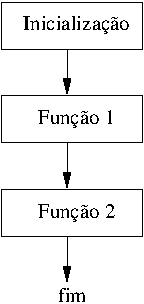
\includegraphics[scale=.6]{fig/seq_app}
	\label{fig:sequential}}} &
	\subfigure[] {
	\fbox{
	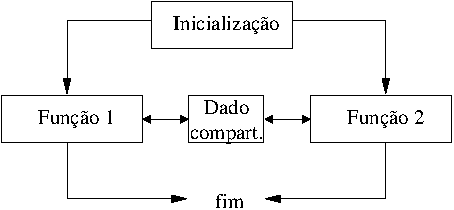
\includegraphics[scale=.6]{fig/par_app}
	\label{fig:parallel}}} &
	\subfigure[] {
	\fbox{
	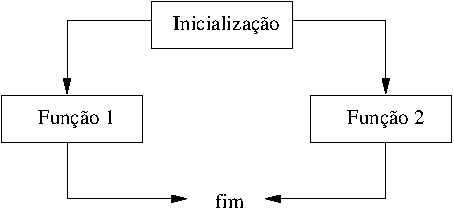
\includegraphics[scale=.6]{fig/best_case_app}
	\label{fig:best-case_app}}}\\
\end{tabular}
\caption{Aplicações do \emph{benchmark}: (a) sequencial (b) paralela (c) melhor-caso.}
\label{fig:apps}
\end{figure}

\prg{app_loop}{Parte do código fonte das aplicações sequencial e paralela.}

A interface de mediadores proposta e o \emph{benchmark} foram implementados no \textsc{EPOS}\footnote{\textsc{EPOS} está disponível online no endereço \url{http://epos.lisha.ufsc.br}.}~\cite{Froehlich:2001}. As 3 aplicações possuem dois arrays bi-dimensionais com tamanho variável (ROWS x COLS) e um laço de 10000 repetições (veja Figura~\ref{prg:app_loop}). O escalonador utilizado nos experimentos foi o CPU\_Affinity, no qual cada thread possui uma afinidade com um \textit{core}. Todos os testes foram executados no processador Intel Core 2 Q9550 (Tabela~\ref{tab:q9550}).

\begin{table}[ht]
\begin{center}
\scriptsize{
\begin{tabular}{|c|c|}
\hline
\multicolumn{2}{|c|}{\textbf{Intel Core 2 Q9550}}\\
\hline
Frequência 			& 2.83 Ghz \\
\hline
Conjunto de instruções	& 64 bits \\
\hline
Número de cores 		& 4 (2 dual-core) \\
\hline
Velocidade do barramento 			& Front-side bus 1.3 Ghz \\
\hline
Cache nível 1 privada (L1) 	& 64 KB 8-way set associative \\
\hline
Tamanho da cache L2 		& 12 MB (2x 6 MB) 24-way set associative\\ 
\hline
Tamanho da linha de cache 	& 64 bytes \\
\hline
Arquitetura de memória	& UMA\\
\hline
Protocolo de coerência 	& MESI \\
\hline
Versão da PMU 	& 2 \\
\hline
Microarquitetura 	& Intel Core Microarchitecture\\
\hline
\end{tabular}
}
\end{center}
\caption{Configuração do processador Intel Core 2 Q9550.}
\label{tab:q9550}	
\end{table}

Primeiramente, a média de 10 execuções de cada aplicação foi medida. A Figura~\ref{fig:avg_execution_time} apresenta os valores obtidos através do componente \texttt{Chronometer} em escala logarítmica para cada versão. As dimensões dos dois arrays (ROWS x COLS) foram configuradas em 64x64 (32~KB), 128x128 (128~KB), 256x256 (512~KB), 512x512 (2~MB), 1024x1024 (8~MB), 1536x1024 (12~MB), e 1536x1536 (18~MB) que excede o tamanho da cache L2 (12~MB). O desvio padrão apresentou uma variação entre 0,01\% e 1\% do total do tempo de execução. É possível notar que o tempo de execução da versão paralela é sempre superior ao da versão sequencial, até 1,55 vez mais lenta. Devido ao compartilhamento dos dados e consequentemente a invalidações da mesma linha de cache realizadas pelo protocolo de coerência, o tempo de execução da versão paralela é afetado. Como esperado, a versão de melhor-caso foi cerca de 2 vezes mais rápida que a sequencial. As linhas 9, 10, 13 e 14 da Figura~\ref{prg:app_loop} são as responsáveis por gerar as transações no barramento que aumentam o tempo de execução.

\fig{avg_execution_time}{Tempo de execução do \emph{benchmark} para cada tamanho dos arrays.}{scale=1}

Com isso é possível constatar que o tempo de execução das aplicações pode ser afetado pela arquitetura dos processadores \emph{multicore} atuais e, em caso de aplicações com restrições de tempo, \emph{deadlines} podem ser perdidos. Assim, é extremamente desejável que o SO seja capaz de monitorar e detectar em tempo real quando atividades que geram disputa por recursos compartilhados aconteçam, a fim de tomar decisões para que o desempenho das aplicações não seja tão degradado. Portanto, a família de mediadores de hardware proposta neste artigo é adequada para este fim. 

Neste sentido, o próximo experimento realizado exemplifica o uso da interface para medir o efeito de excessivas invalidações da mesma linha de cache no hardware. O evento medido foi o CMP\_SNOOP. Esse evento conta o número de vezes que dados presentes na cache L1 de um \textit{core} são requisitados (\textit{snooped}) por outro. Um \textit{snoop} é realizado através de uma porta de escrita na cache de dados L1. Consequentemente, frequentes \textit{snoops} podem conflitar com escritas à cache de dados L1 e assim aumentar a latência e impactar o desempenho~\cite{intelsys}. A Figura~\ref{prg:api_example} mostra parte do código fonte das aplicações utilizando o componente de monitoramento de desempenho (\emph{Perf\_Mon}) que faz uso do mediador de hardware implementado. As chamadas aos métodos de configuração (\emph{l1\_data\_cache\_snooped}) e leitura (\emph{get\_l1\_data\_cache\_snooped}) do evento são diluídas em tempo de compilação no código das aplicações, assim nenhuma chamada de método é gerada na imagem final do sistema.

\prg{api_example}{Exemplo de como a API foi utilizada nos experimentos nas aplicações paralela e melhor-caso.}

A Figura~\ref{fig:l1_data_cache_snooped} mostra o número de eventos mensurados para cada versão do \emph{benchmark} e para cada tamanho dos arrays. O evento foi configurado para contar os \textit{snoops} que geram invalidações da mesma linha de cache. Uma invalidação em uma linha de cache acontece quando o \textit{core} não possui aquela linha ou quando a linha está disponível somente para leitura e o outro \textit{core} deseja escrever nessa linha. Basicamente, as linhas 13 e 14 do código fonte da Figura~\ref{prg:app_loop} são responsáveis pelas invalidações mensuradas por este evento. 

\fig{l1_data_cache_snooped}{Número de \textit{snoops} de uma linha de cache. O evento CMP\_SNOOP foi configurado para contar os \textit{snoops} de invalidação de todos \textit{cores}.}{scale=1}

A versão paralela apresentou de 2 a 3 ordens de magnitude mais \textit{snoops} que as versões sequencial e melhor-caso. Quando o tamanho dos dados é maior que a cache L2 (de 12~MB a 18~MB), a versão paralela apresentou uma pequena queda no número de \textit{snoops} devido ao fato de que existem mais dados sendo substituídos na cache (e.g., conflitos pela mesma linha de cache) e assim a probabilidade de um dado requisitado não estar na cache é menor. O desvio padrão do melhor-caso variou de 10\% para 32~KB e 128~KB a 0,05\% para 18~MB. O desvio padrão máximo para as versões sequencial e paralela foi 4,82\% para tamanho de 2~MB e 3,49\% para 62~KB respectivamente. O número total de \textit{snoops} representa de 0,04\% a 1,67\% do total de escritas realizadas pelo código em um \textit{core} para a versão paralela e cerca de 0,0005\% para as versões sequencial e melhor-caso. Os \textit{snoops} mensurados nas versões sequencial e melhor-caso são resultado das variáveis de controle (\textit{spinlocks}) necessárias em um kernel \emph{multicore}.. As linhas 13 e 14 da Figura~\ref{prg:app_loop} são responsáveis pelas escritas que geram o evento medido. As leituras não são consideradas pois elas não geram transações de invalidações no barramento. É importante salientar que nem toda escrita ou leitura de um dado vai gerar um \textit{snoop} no barramento. Dependendo do estado da linha da cache em um \textit{core} (dado pelo protocolo de coerência), uma ação é tomada pelo controlador de memória. Por exemplo, considerando o protocolo de coerência MESI, se a linha de cache em um \textit{core} está no estado E (exclusivo) e uma requisição para leitura é vista no barramento, este \textit{core} deve mudar a linha para o estado S (compartilhado). Por outro lado, se um \textit{core} escreve em uma linha de cache no estado E ou M, nenhuma transação no barramento é gerada pois esta linha só está presente na cache daquele \textit{core}. Invalidações da linha de cache acontecem apenas em escritas nas linhas de cache compartilhadas (estado S) ou inválidas (estado I).

Os valores medidos na Figura~\ref{fig:l1_data_cache_snooped} foram então normalizados em um período de 10~ms dado pela Equação~\ref{eq:norm}:

\begin{equation}
 N = \frac{AVG_s}{AVG_{ex} / 10 ms} 
\label{eq:norm}
\end{equation}

Onde $AVG_s$ é a média de \textit{snoops} e $AVG_{ex}$ é a média do tempo de execução. A Figura~\ref{fig:l1_data_cache_snooped_period} mostra os valores normalizados para cada aplicação e tamanho dos dados. Nota-se que praticamente não existe variação para as aplicações sequencial e melhor-caso, cerca de 60 a 80 \textit{snoops} em um período de 10~ms. A versão paralela apresentou até 100.000 \textit{snoops} em um período. Esse gráfico mostra a frequência de invalidações de uma linha da cache e como um evento de hardware pode ser utilizado pelo SO. Por exemplo, durante um quantum de escalonamento, esse evento poderia ser monitorado e se o valor mensurado fosse maior que um valor limite, o escalonador poderia tomar uma decisão de escalonar ou não uma thread, movê-la para o mesmo \textit{core} de outra ou ainda diminuir o grau de paralelismo para diminuir a disputa pelos dados compartilhados.

\fig{l1_data_cache_snooped_period}{Número de \textit{snoops} de uma linha de cache em um período de 10~ms.}{scale=1}

A API proposta foi implementada em C++ em sistema operacional baseado em componentes (\textsc{EPOS}). Sendo assim, a mesma infra-estrutura de mediadores e componentes poderia ser facilmente utilizada por qualquer outro sistema operacional baseado em componentes e implementado em C++. 

\section{Trabalhos Relacionados}
\label{sec:rel}

PAPI (\emph{Performance API}) é a interface de código aberto mais utilizada para monitoramento de desempenho através de HPCs~\cite{Dongarra:2003,papi}. PAPI consiste de uma camada independente de plataforma, uma interface de alto nível que provê comandos como leitura, inicialização e parada dos contadores e uma interface de baixo nível que disponibiliza mais funcionalidades aos desenvolvedores. Essa camada de baixo nível poderia ser comparada aos mediadores de hardware propostos neste artigo. Entretanto, não é objetivo nesse trabalho, fazer uma comparação entre as duas implementações. PAPI suporta uma grande variedade de arquiteturas, tendo sido projetada para sistemas computacionais de propósito geral e está em desenvolvimento por mais de 10 anos. A interface proposta, ao contrário, foi projetada para aplicações embarcadas que possuem seus requisitos conhecidos em tempo de projeto. Assim, é possível gerar somente o código necessário para a aplicação, economizando recursos e deixando a comunicação entre software e hardware mais rápida.
 
O \textsc{Linux} abstrai o uso de HPCs através de um subsistema de contadores de desempenho. A ferramenta \emph{perf}, disponível juntamente com o código fonte do SO, usa esse subsistema e permite que desenvolvedores obtenham e analisem o desempenho de suas aplicações. Outras ferramentas como a Intel \textsc{Vtune}~\cite{intelperf} e AMD \textsc{CodeAnalyst}~\cite{codeanalyst} oferecem uma interface gráfica ``amigável'' para monitorar o desempenho de processadores e aplicação através de HPCs. Entretanto, SETR geralmente não apresentam uma interface entre o desenvolvedor/usuário e o sistema em si.

Existem trabalhos que utilizam HPCs juntamente com o escalonador do SO para dinamicamente tomar decisões como mover threads de um \textit{core} para outro. Bellosa e Steckermeier foram os primeiros autores a usar HPCs com esse propósito~\cite{Bellosa:1996}. Weissman usa HPCs para monitorar o número de cache \textit{misses} em um quantum de escalonamento e, juntamente com anotações do desenvolvedor no código fonte, montar um grafo representando as dependências do estado da cache entre as threads~\cite{Weissman:1998}. O objetivo é avaliar os efeitos do tamanho dos dados das threads na cache de um processador. Com base no modelo, são propostas duas políticas de escalonamento, porém elas não consideram invalidações na mesma linha de cache devido ao compartilhamento de dados.

Tam et al. usaram HPCs para monitorar os endereços de linhas de cache que são invalidados devido à coerência de cache. Uma estrutura de dados que contém os endereços lidos é construída para cada thread do sistema~\cite{Tam:2007}. Usando as informações desta estrutura, o escalonador monta um grupo composto por um conjunto de threads e aloca este grupo a um \textit{core} específico. West et al. propuseram uma técnica baseada em um modelo estatístico para estimar a ocupação da cache por cada thread do sistema em tempo de execução~\cite{West:2010}. No entanto, compartilhamento de dados entre as threads também não é considerado pelos autores.

Zhuravlev identifica os principais problemas que causam contenção em processadores \emph{multicore}: contenção pelo controlador de memória, barramento de memória, hardware \textit{prefetching} e espaço da cache~\cite{Zhuravlev:2010}. Os autores ainda propõem dois algoritmos de escalonamento que usam a taxa de \textit{miss} da cache para distribuir as threads de forma equilibrada entre os \textit{cores} e assim diminuir esta taxa e aumentar o desempenho das aplicações. Calandrino e Anderson também utilizam o número de \textit{misses} da cache para estimar o tamanho dos dados de cada thread~\cite{Calandrino:2009}. Baseando-se nesse número estimado, um escalonador de tempo real e consciente do tamanho da cache, escalona as threads nos \textit{cores} de maneira que não causem \textit{thrashing} na cache compartilhada.

\section{Considerações Finais}
\label{sec:conc}

Este artigo apresentou o projeto de uma família de mediadores de hardware para unidades de monitoramento de desempenho presentes nos processadores atuais, dentro do contexto de sistemas embarcados. O código gerado pelos mediadores é diluído em tempo de compilação nos componentes que os utilizam. Assim, é obtido um baixo consumo de memória e um bom desempenho, características desejáveis para um sistema embarcado. Com o intuito de demonstrar a utilização dos mediadores propostos, um \emph{benchmark} que compartilha dados entre duas threads foi implementado e os mediadores propostos foram usados para prover ao sistema operacional uma visão da relação entre o software em execução e os eventos gerados no hardware por esse software.

Como trabalhos futuros, pretendemos utilizar o suporte a HPCs juntamente com o escalonador para garantir o atendimento aos \emph{deadlines} em aplicações embarcadas de tempo real. Um componente independente de plataforma responsável por agregar funcionalidades à família de mediadores de PMU também será alvo de implementação futura.

\section*{Agradecimentos}

Este trabalho foi financiado parcialmente pela CAPES, projeto RH-TVD 006/2008.


\bibliographystyle{sbc}
\bibliography{references}

\end{document}
